\documentclass[conference]{IEEEtran}
\IEEEoverridecommandlockouts
% The preceding line is only needed to identify funding in the first footnote. If that is unneeded, please comment it out.
\usepackage{cite}
\usepackage{amsmath,amssymb,amsfonts}
\usepackage{algorithmic}
\usepackage{graphicx}
\usepackage{textcomp}
\usepackage{xcolor}
\usepackage{ctex}
\usepackage{fontspec}
\usepackage{listings}
\usepackage{pxfonts}
\def\BibTeX{{\rm B\kern-.05em{\sc i\kern-.025em b}\kern-.08em
    T\kern-.1667em\lower.7ex\hbox{E}\kern-.125emX}}

\begin{document}

\title{傅立叶变换光谱测量技术实验报告}

\author{
    \IEEEauthorblockN{
        黄润华}
        \IEEEauthorblockA{
            \textit{Ocean University of China} \\
            \textit{email@noreply.com}
    \and
    \IEEEauthorblockN{
        杨超}
        \IEEEauthorblockA{
            \textit{Ocean University of China} \\
            \textit{email@somewhere.com}
        }
    }
}
\maketitle

\begin{abstract}
    本实验报告为傅立叶变换光谱测量技术第四次实验报告,本报告采用Python仿真同时考虑有限扫描长度和采样间隔误差两因素影响下的傅里叶变换光谱测量系统的光谱测量曲线。实验仿真误差选取是随机、线性或正弦变化的误差,仿真采样间隔为79.1nm。本仿真以632.8nm的HeNe激光和532nm的YAG激光为例。
\end{abstract}

\begin{IEEEkeywords}
    Optical spectrum, python, fft
\end{IEEEkeywords}

\section{实验目的}
\begin{itemize}
    \item[1.] 仿真多种正弦形式的扫描长度误差与采样间隔误差同时叠加对傅里叶变换光谱测量曲线的影响。
    \item[2.] 仿真扫描长度误差与采样间隔误差累积叠加对傅里叶变换光谱测量曲线的影响。
\end{itemize} 

\section{实验原理}
\subsection{单色线的干涉方程}
理论上单色线的干涉图可以用公式(\ref{eq1})来描述
\begin{align}
    I(x) = 2cos(2\pi \sigma_0 x)    \label{eq1}
\end{align}

\subsection{采样间隔误差对干涉方程的影响}
人为进行动镜的平移过程通常掺杂着过程噪声。过程噪声的形式多种多样,常见的简单过程噪声类型为正弦噪声、随机噪声与线性噪声。然而,外部环境是一个不可预测的变量,在不同时刻的噪声类型通常是不相关且随机的,这种随机性带给光谱测量的影响是复杂性的。在操作不当的情况下,动镜移动的距离受到过程噪声的影响较大时,得到的傅立叶变换光谱测量曲线具备较低的可信度同时带来了阅读上的复杂性。

动镜移动时过程噪声带来的采样间隔误差是不可避免的,采样间隔误差的直接影响主要体现在对公式(\ref{eq1})中扫描长度$x$的影响:
\begin{align}
    I(x) = cos(2\pi\sigma_0(x + \varepsilon_s)) \label{eq9}
\end{align}

采样过程通常会选取$2^{12}$到$2^{20}$个采样点,每次采样均有可能存在一定的采样误差,采样误差经过多次迭代后对最终傅立叶光谱测量曲线带来的影响是可观且巨大的。

本次仿真模拟的采样间隔误差均为简单采样间隔误差,即代表每次采样时的误差类型为单一的正弦噪声误差、随机噪声误差或线性噪声误差。同时假设采样过程均为独立事件,前后采样过程噪声互不相干且独立。

正弦形式的采样间隔误差表达式如下:
\begin{align}
    \varepsilon_s = \frac{\lambda_0}{16}sin(2\pi\sigma_{\varepsilon}x)  \label{eq2}
\end{align}
其中波数(Wave number)数值为$\sigma_{\varepsilon} = 0.4\times10^4 m^{-1}$。

随机形式的采样间隔误差表达式可以采用均匀分布来表示:
\begin{align}
    \varepsilon_s \sim U(-\frac{\lambda_0}{5}, \frac{\lambda_0}{5})   \label{eq3}
\end{align}

线性形式的采样间隔误差表达式可以用正比例函数来表示:
\begin{align}
    \varepsilon_s(k) = k, \;\;\; k \in [0, \;79.1\times10^9 m] \label{eq4}
\end{align}

\section{实验内容}
仿真同时考虑有限扫描长度和采样间隔误差两因素影响下的傅里叶变换光谱测量系统的光谱测量曲线。误差可以是随机、线性或正选变化的。以632.8nm的He-Ne激光和532nm的YAG激光为例。(采样间隔为79.1nm)

\begin{figure*}[htbp]
	\centerline{
		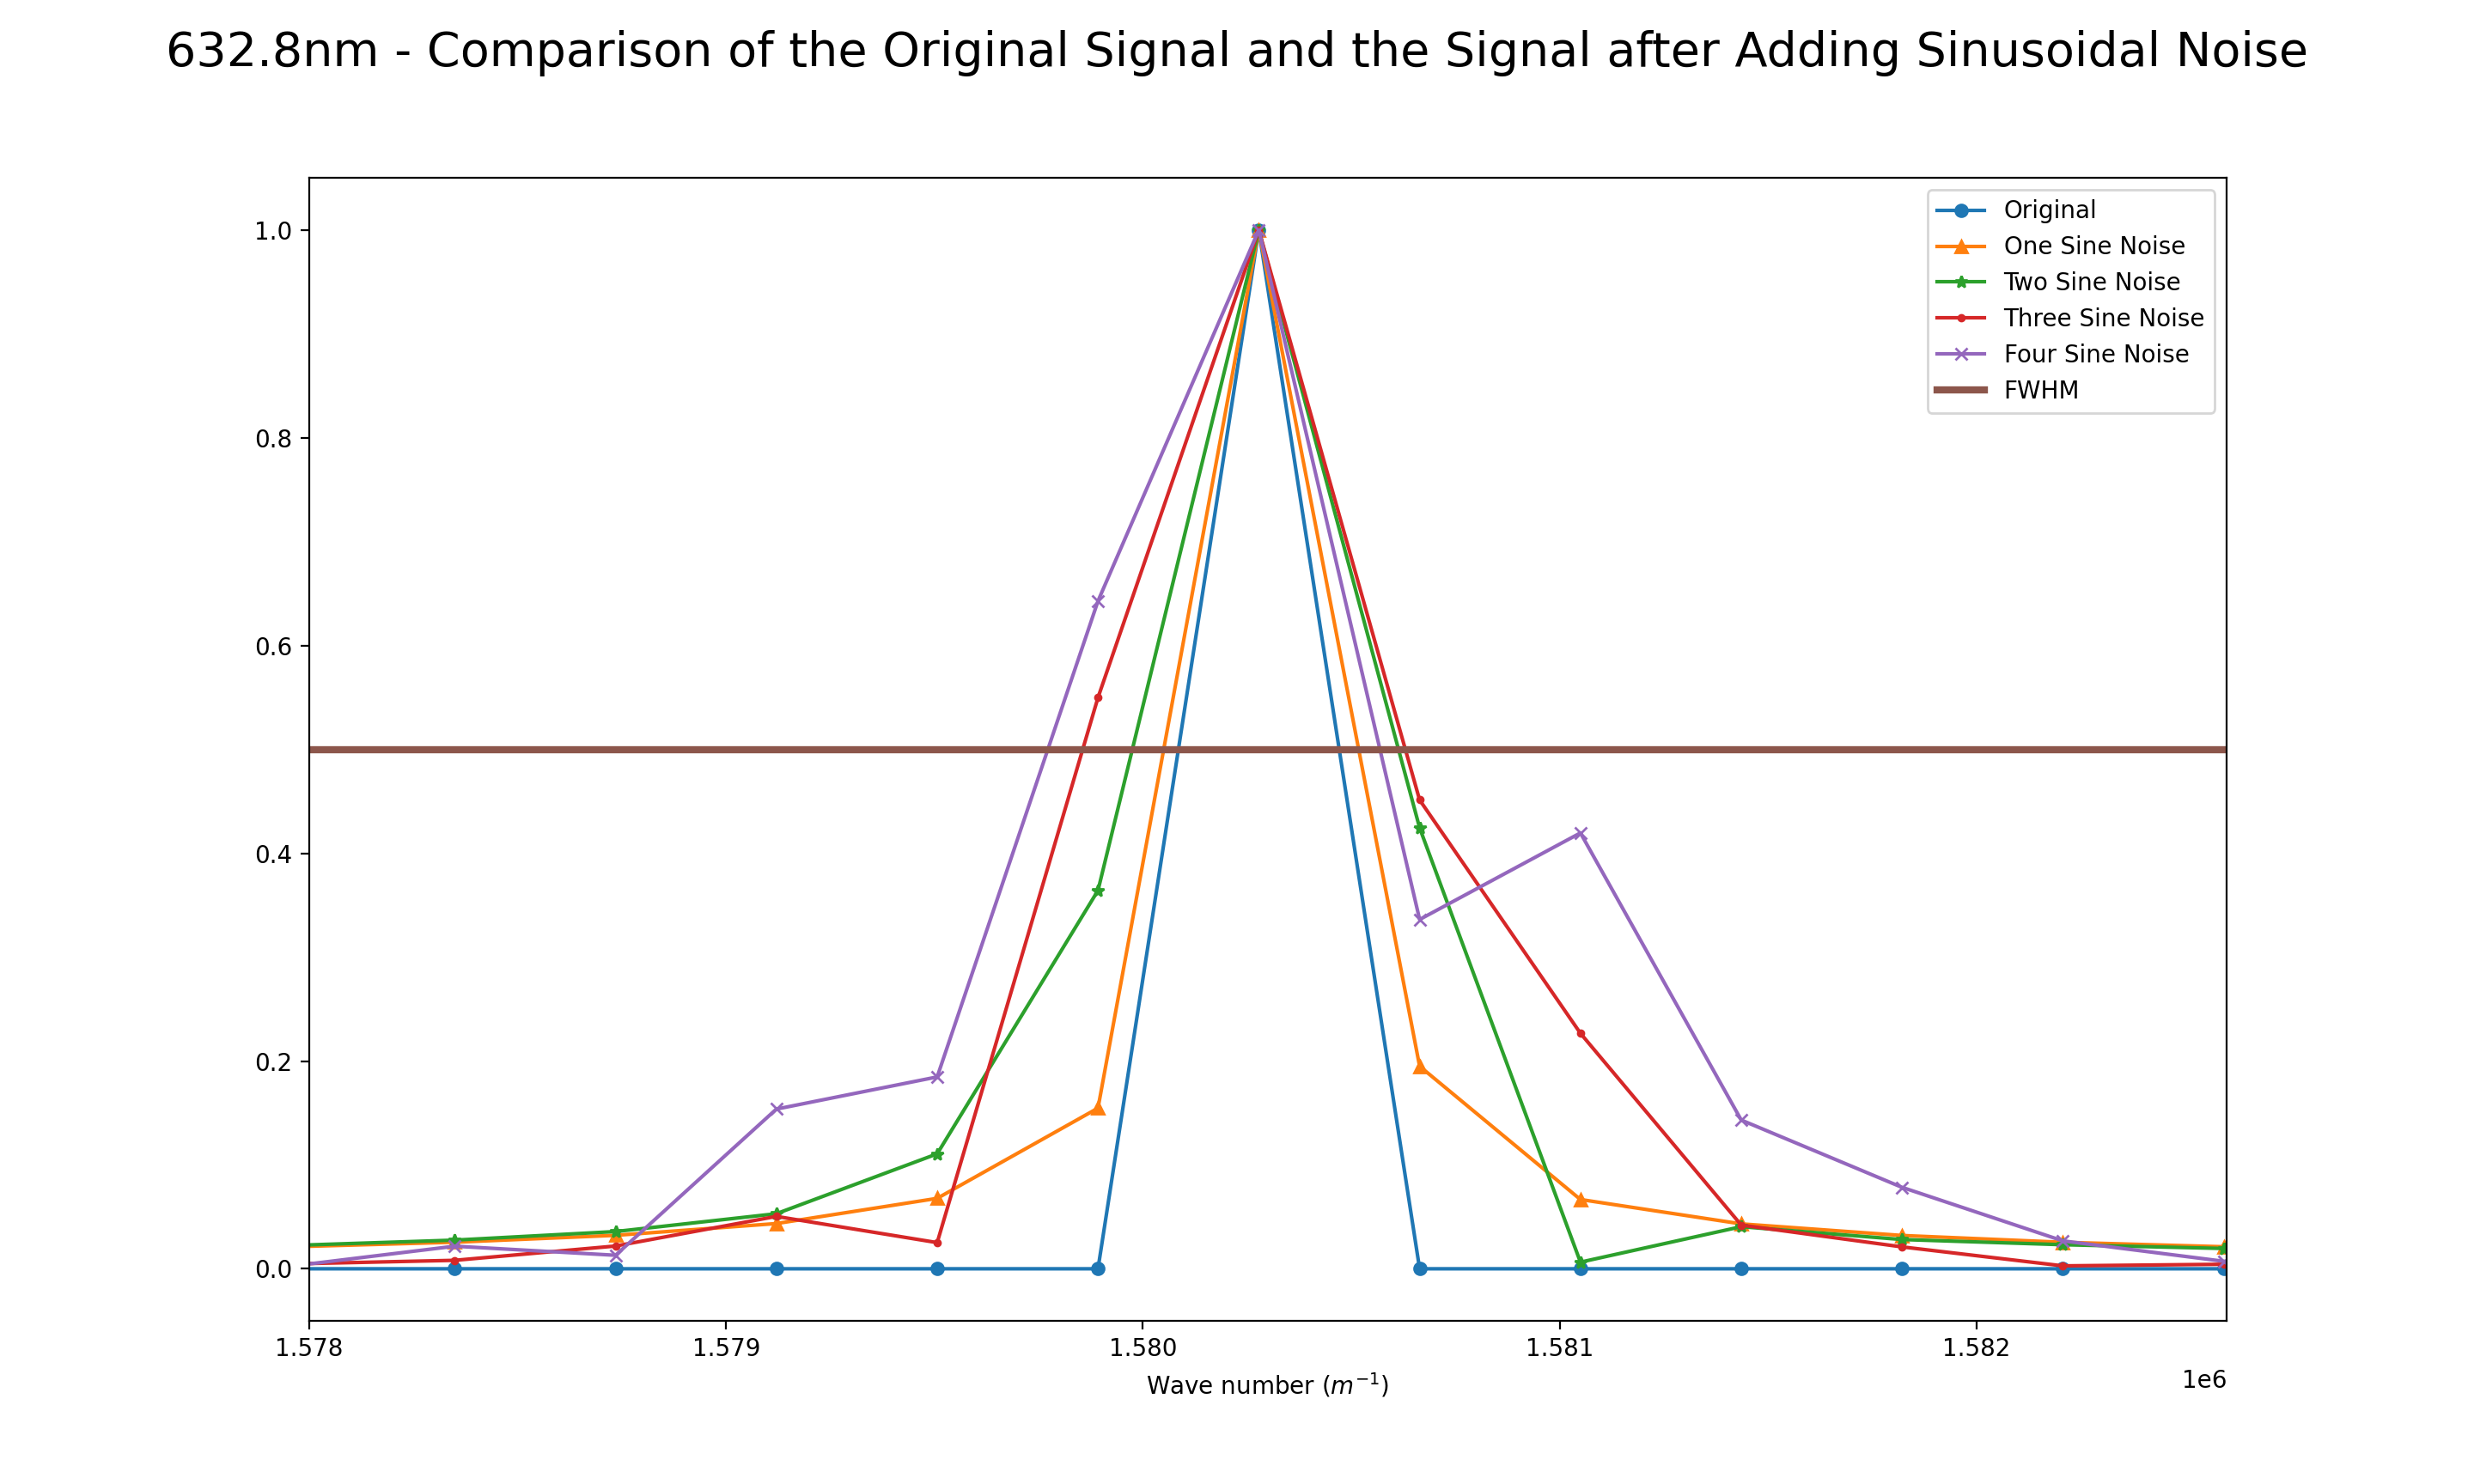
\includegraphics[width=22cm]{所有波放一起.png} 	
	}
	\caption{原始信号的光谱曲线与叠加多种不同频率正弦噪声后光谱曲线的比较}
	\label{pic7}
\end{figure*}

\section{实验结果}
本实验报告分析以632.8nm的波长为例。

\subsection{不同频率正弦波噪声的叠加结果}
图片\ref{pic1}、图\ref{pic2}、图\ref{pic3}与图\ref{pic14}显示了本次仿真的不同频率正弦波噪声,其中图\ref{pic1}为单一频率正弦波噪声叠加后的光谱曲线,图\ref{pic2}为两个不同频率正弦波噪声叠加后的光谱曲线,图\ref{pic3}为三个不同频率正弦波噪声叠加后的光谱曲线,图\ref{pic14}为四个不同频率正弦波噪声叠加后的光谱曲线。从光谱曲线上可以看到,随着叠加的正弦噪声数的增加,光谱曲线的半峰全宽逐渐增大。

\begin{figure}[htbp]
    \centerline{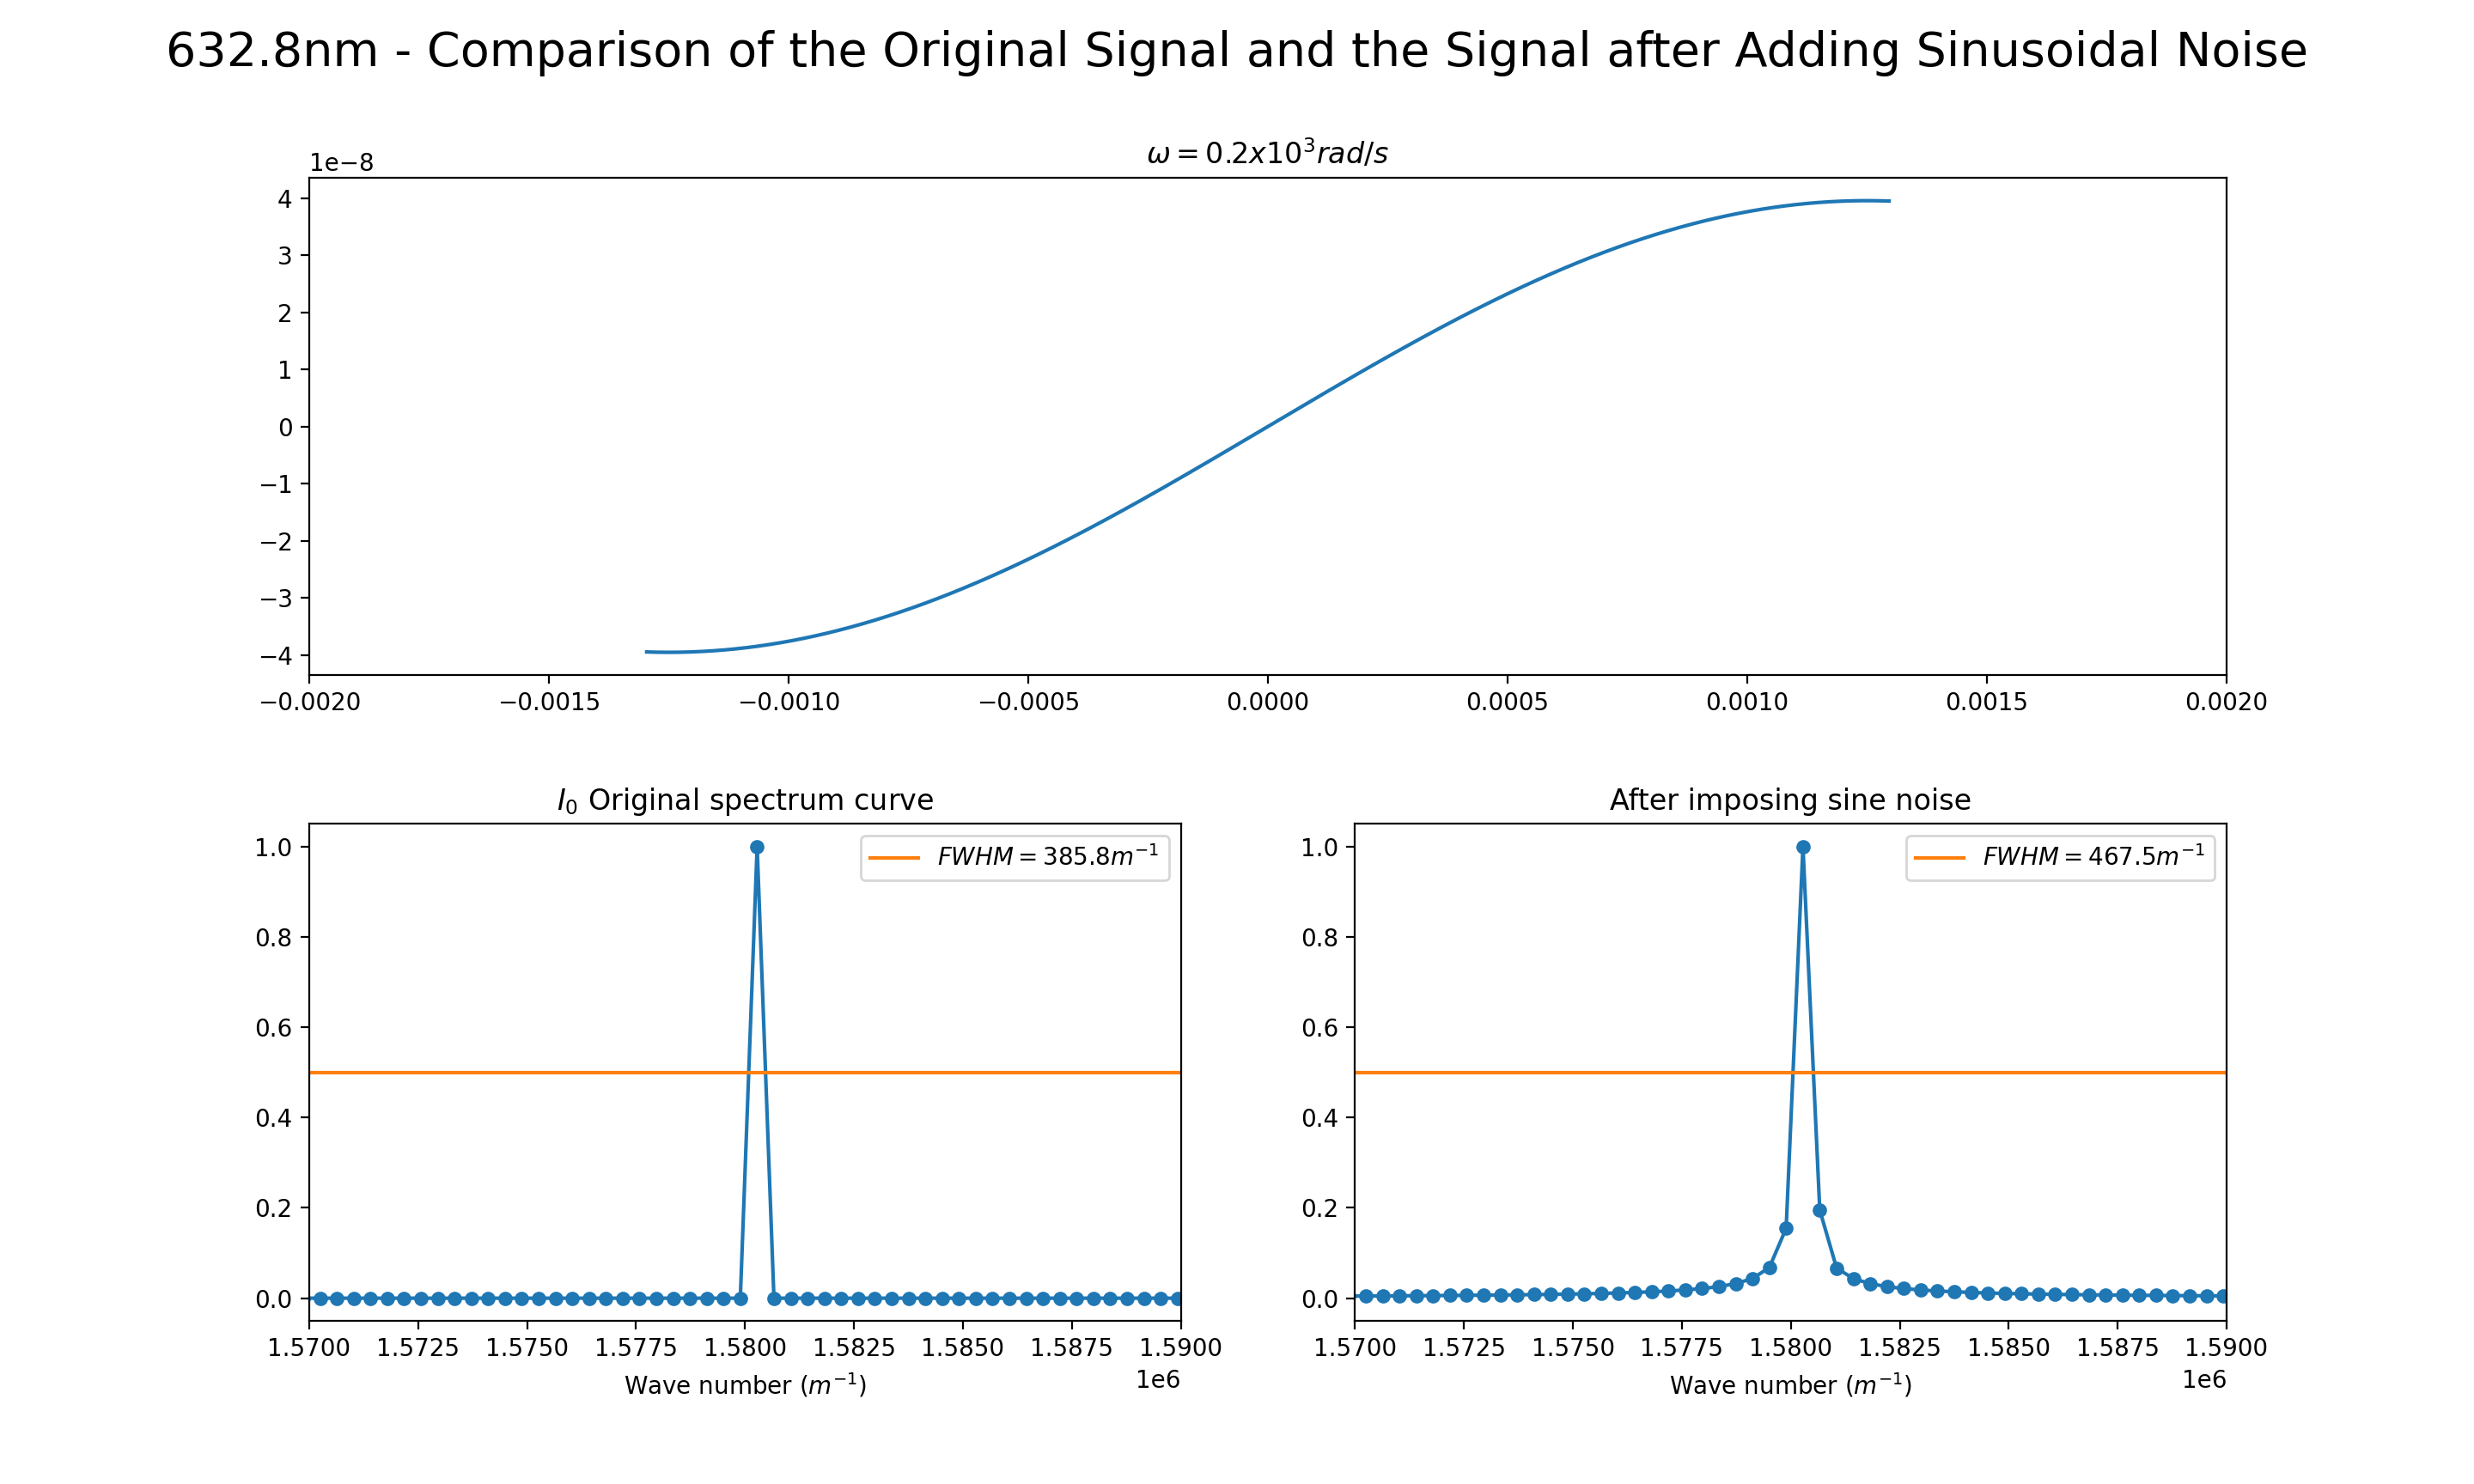
\includegraphics[width=0.5\textwidth]{1种波叠加.png}}
    \caption{单一频率正弦波噪声叠加后的光谱曲线}
    \label{pic1}
\end{figure}

\begin{figure}[htbp]
    \centerline{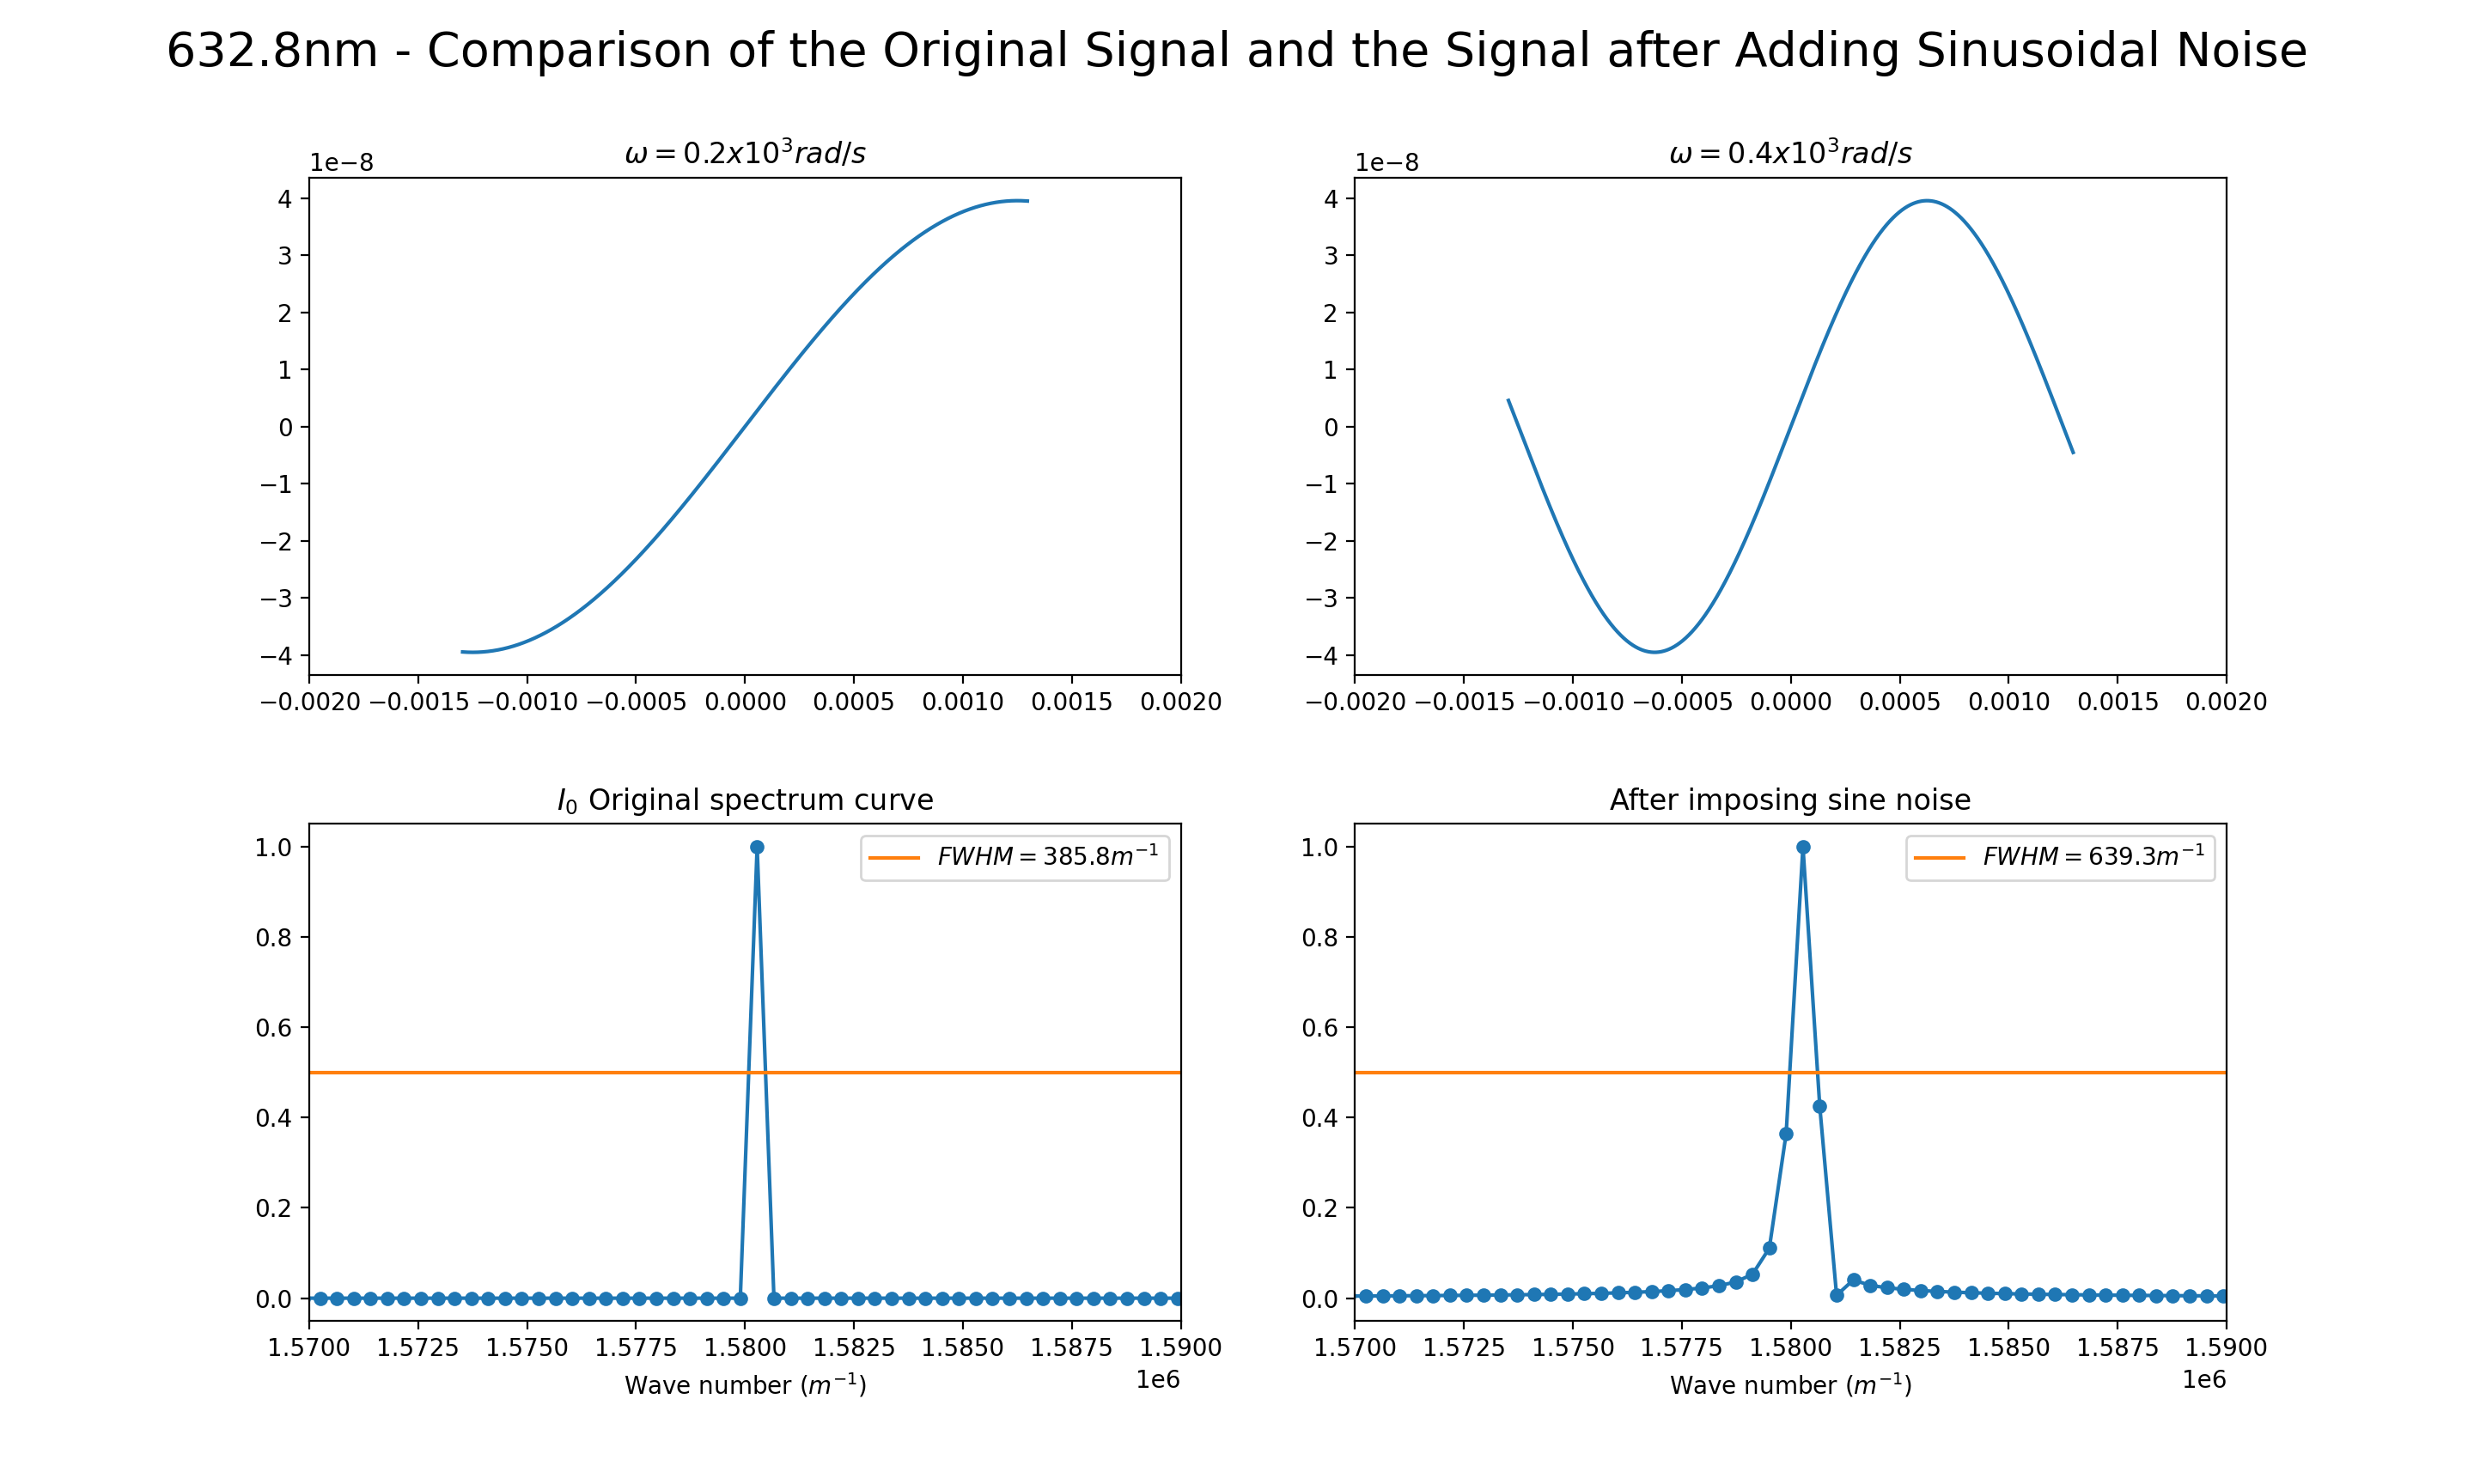
\includegraphics[width=0.5\textwidth]{2种波叠加.png}}
    \caption{两个不同频率正弦波噪声叠加后的光谱曲线}
    \label{pic2}
\end{figure}

\begin{figure}[htbp]
    \centerline{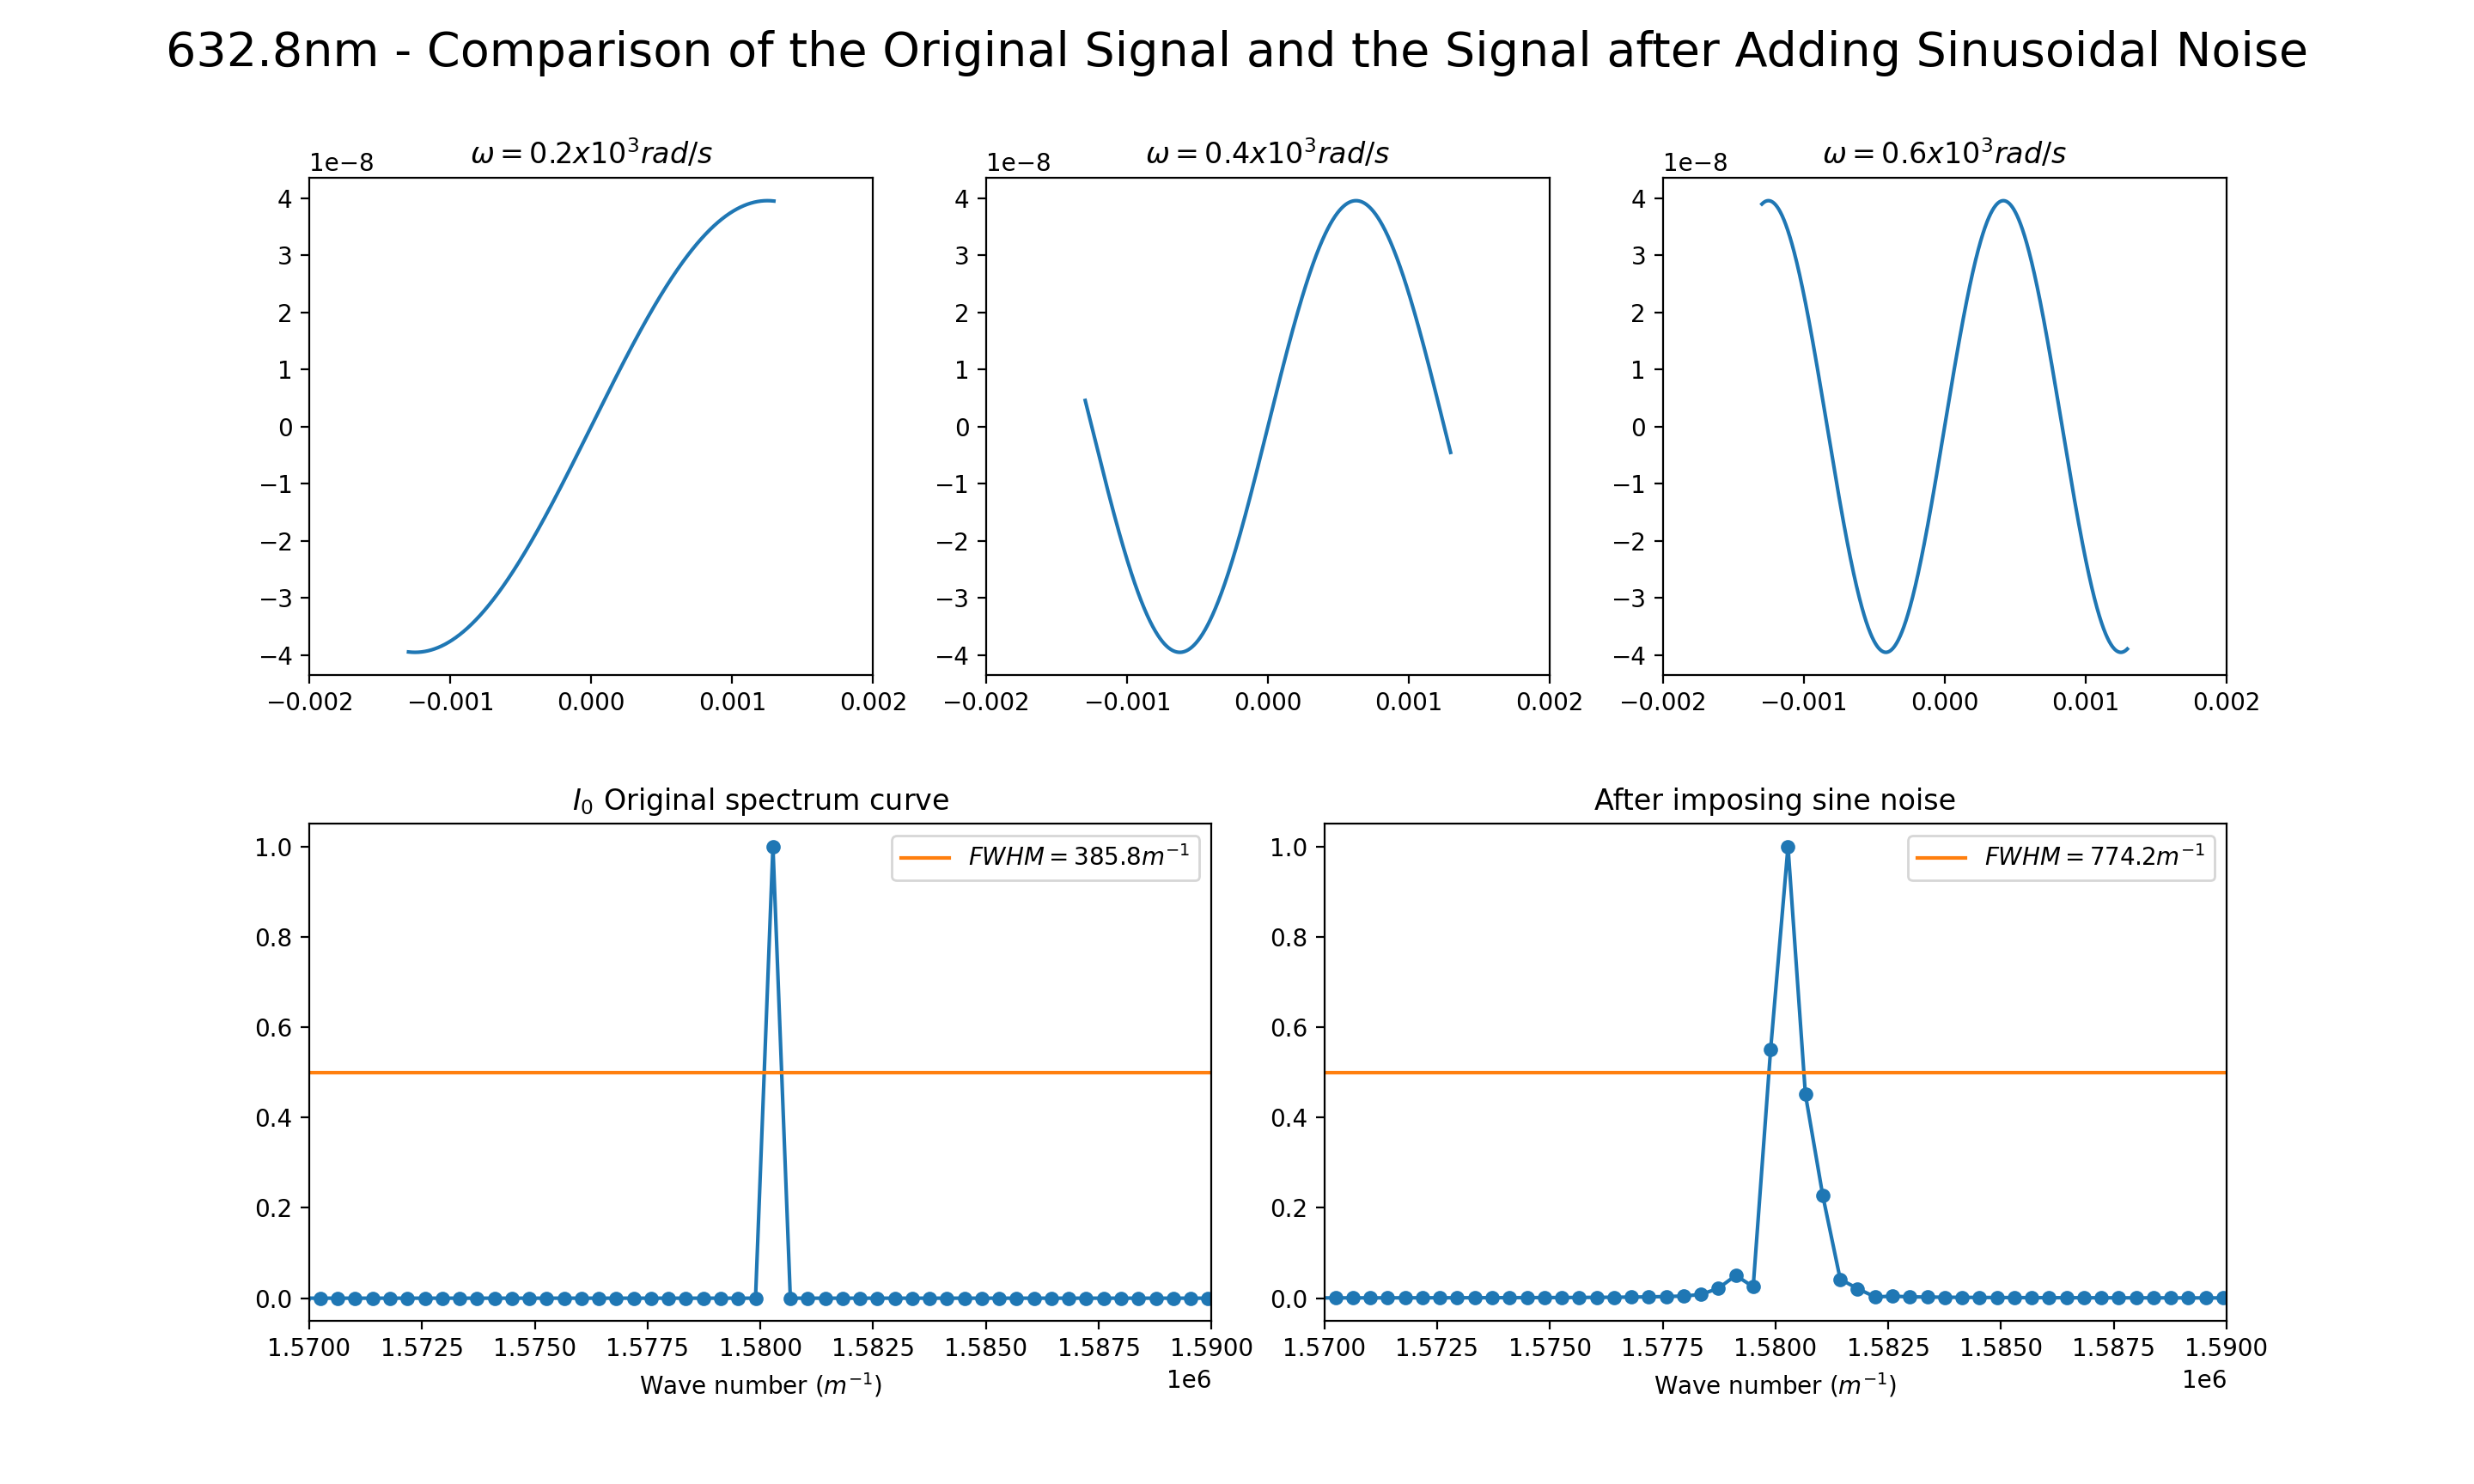
\includegraphics[width=0.5\textwidth]{3种波叠加.png}}
    \caption{三个不同频率正弦波噪声叠加后的光谱曲线}
    \label{pic3}
\end{figure}

\begin{figure}[htbp]
    \centerline{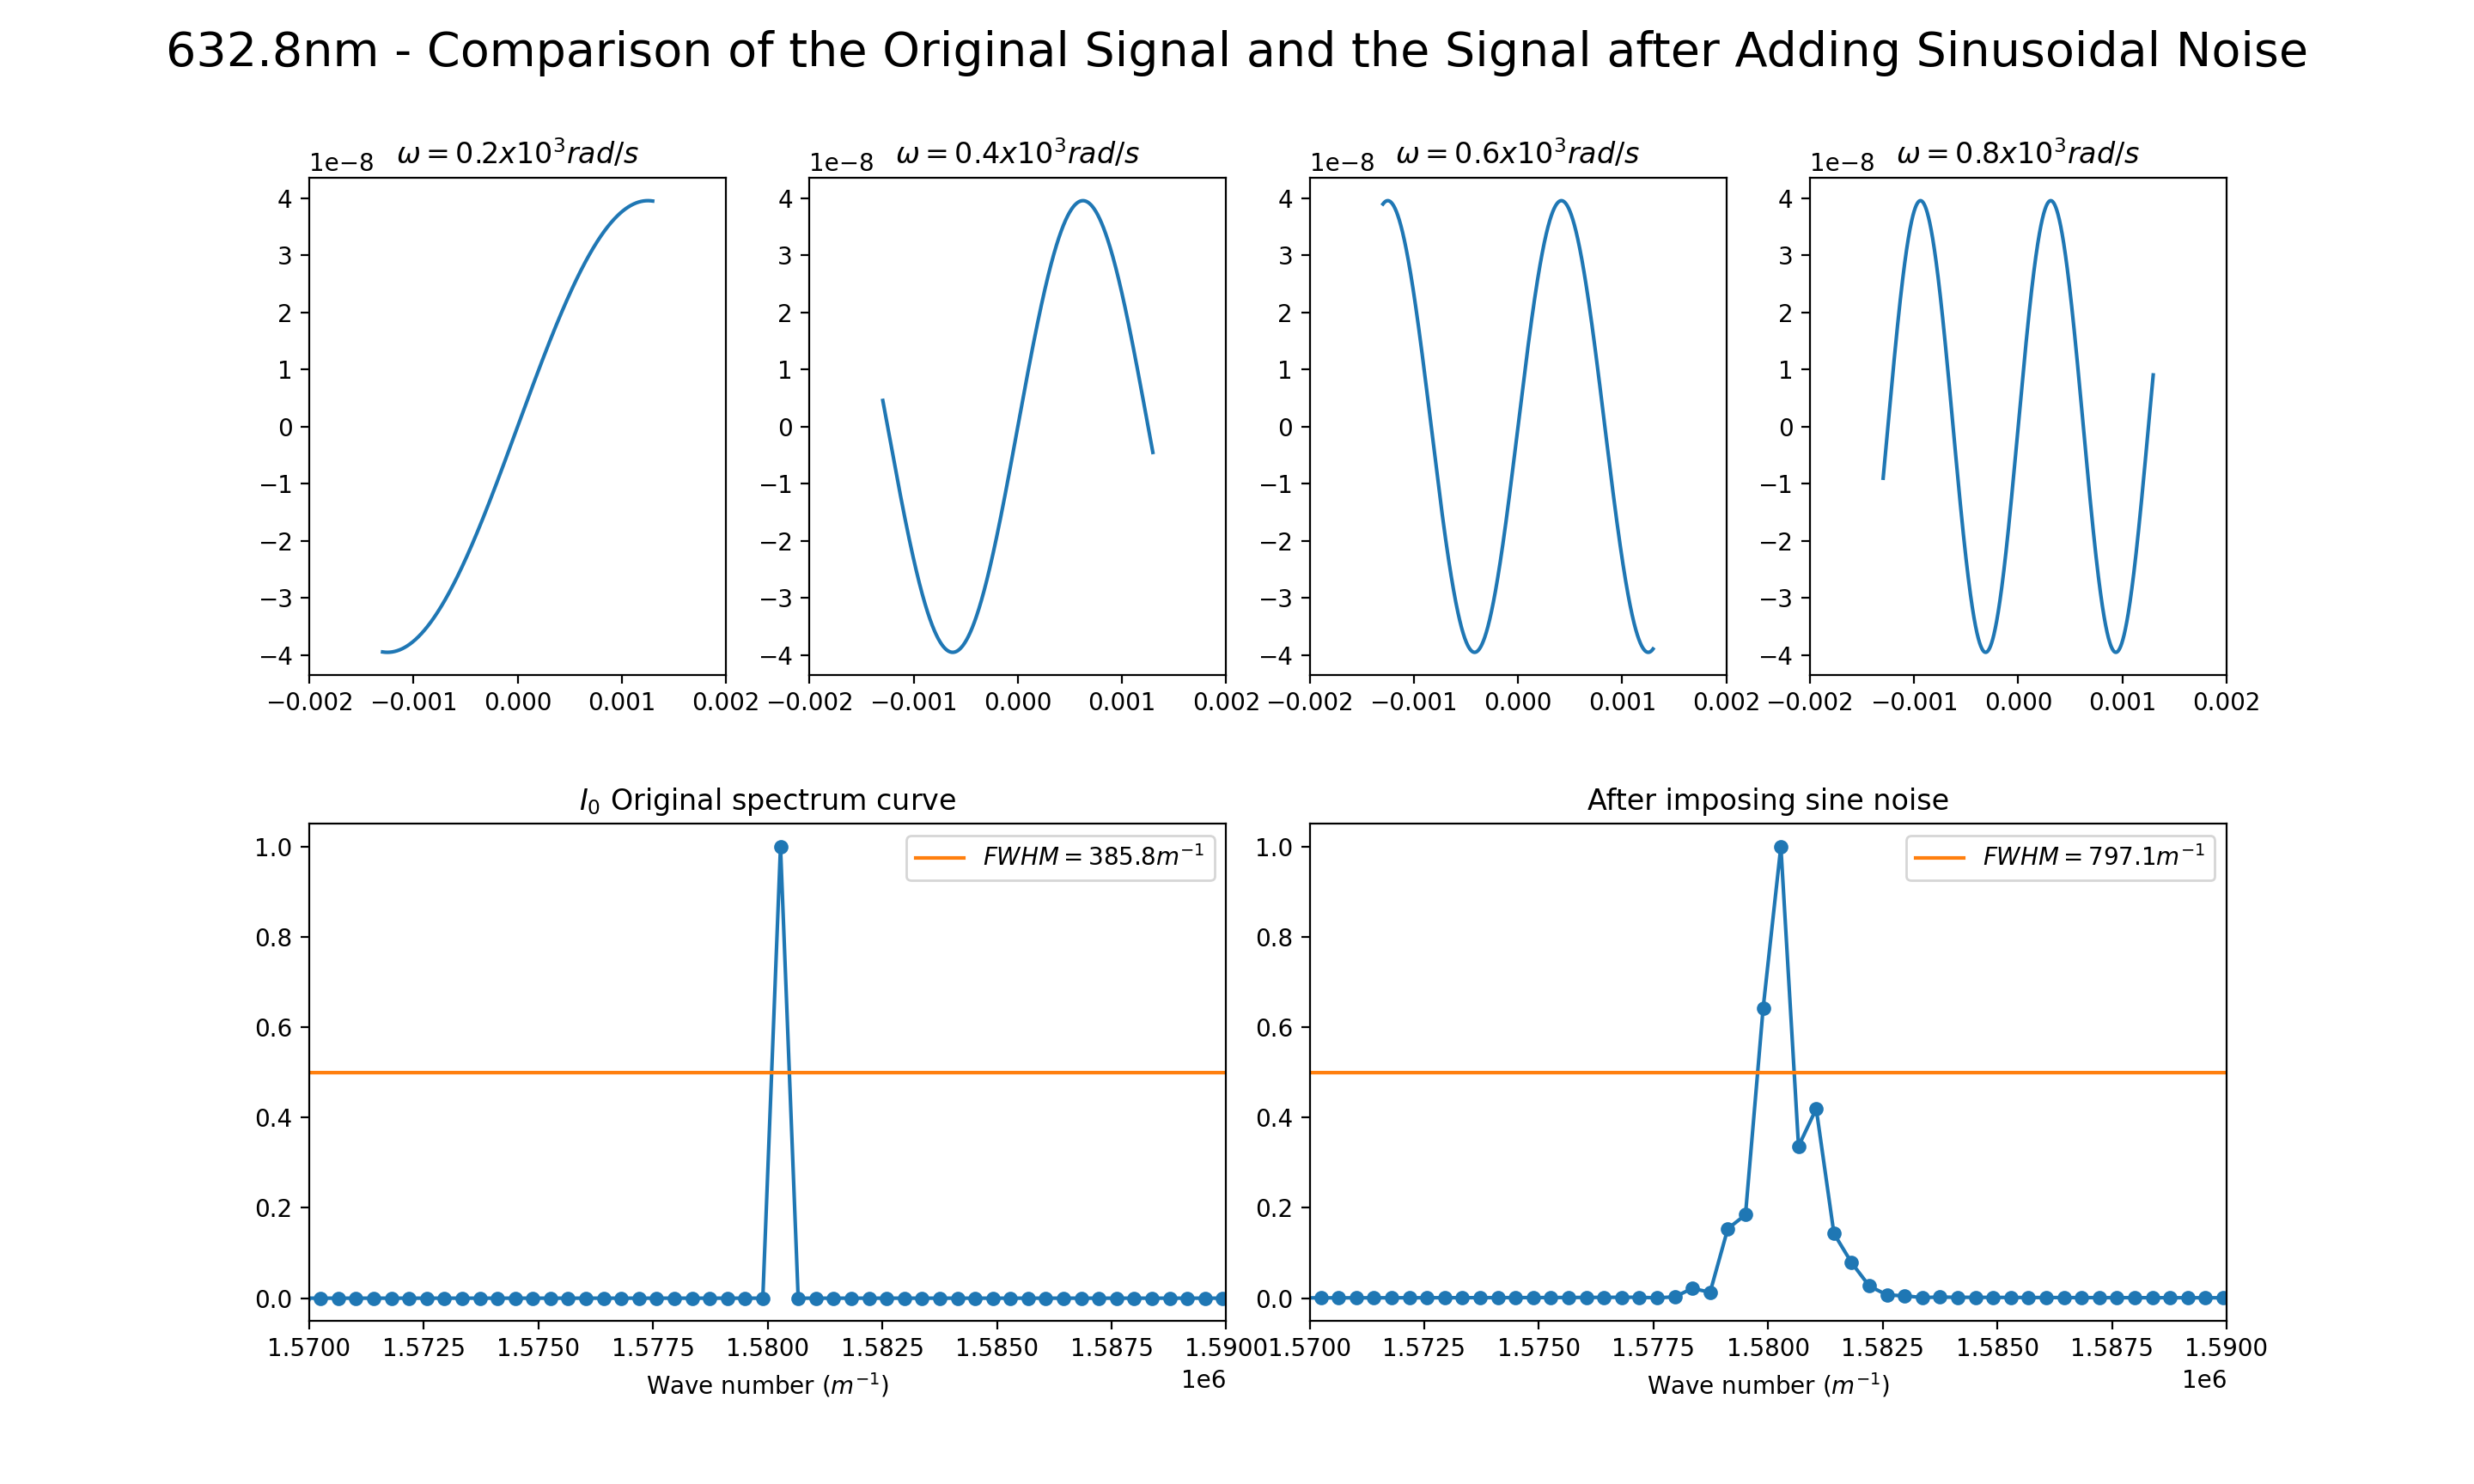
\includegraphics[width=0.5\textwidth]{4种波叠加.png}}
    \caption{四个不同频率正弦波噪声叠加后的光谱曲线}
    \label{pic14}
\end{figure}

\subsection{噪声累积叠加结果}
图片\ref{pic21}、图\ref{pic22}、图\ref{pic23}与图\ref{pic24}显示了四种不同幅度值的随机噪声的累积叠加结果。每张图片第一行代表理论扫描距离与叠加多次噪声后的扫描距离的比较,第二行左半部分代表代表未添加累积噪声的光谱曲线图,右半部分代表添加累积随机噪声后的光谱曲线图。

\begin{figure}[htbp]
    \centerline{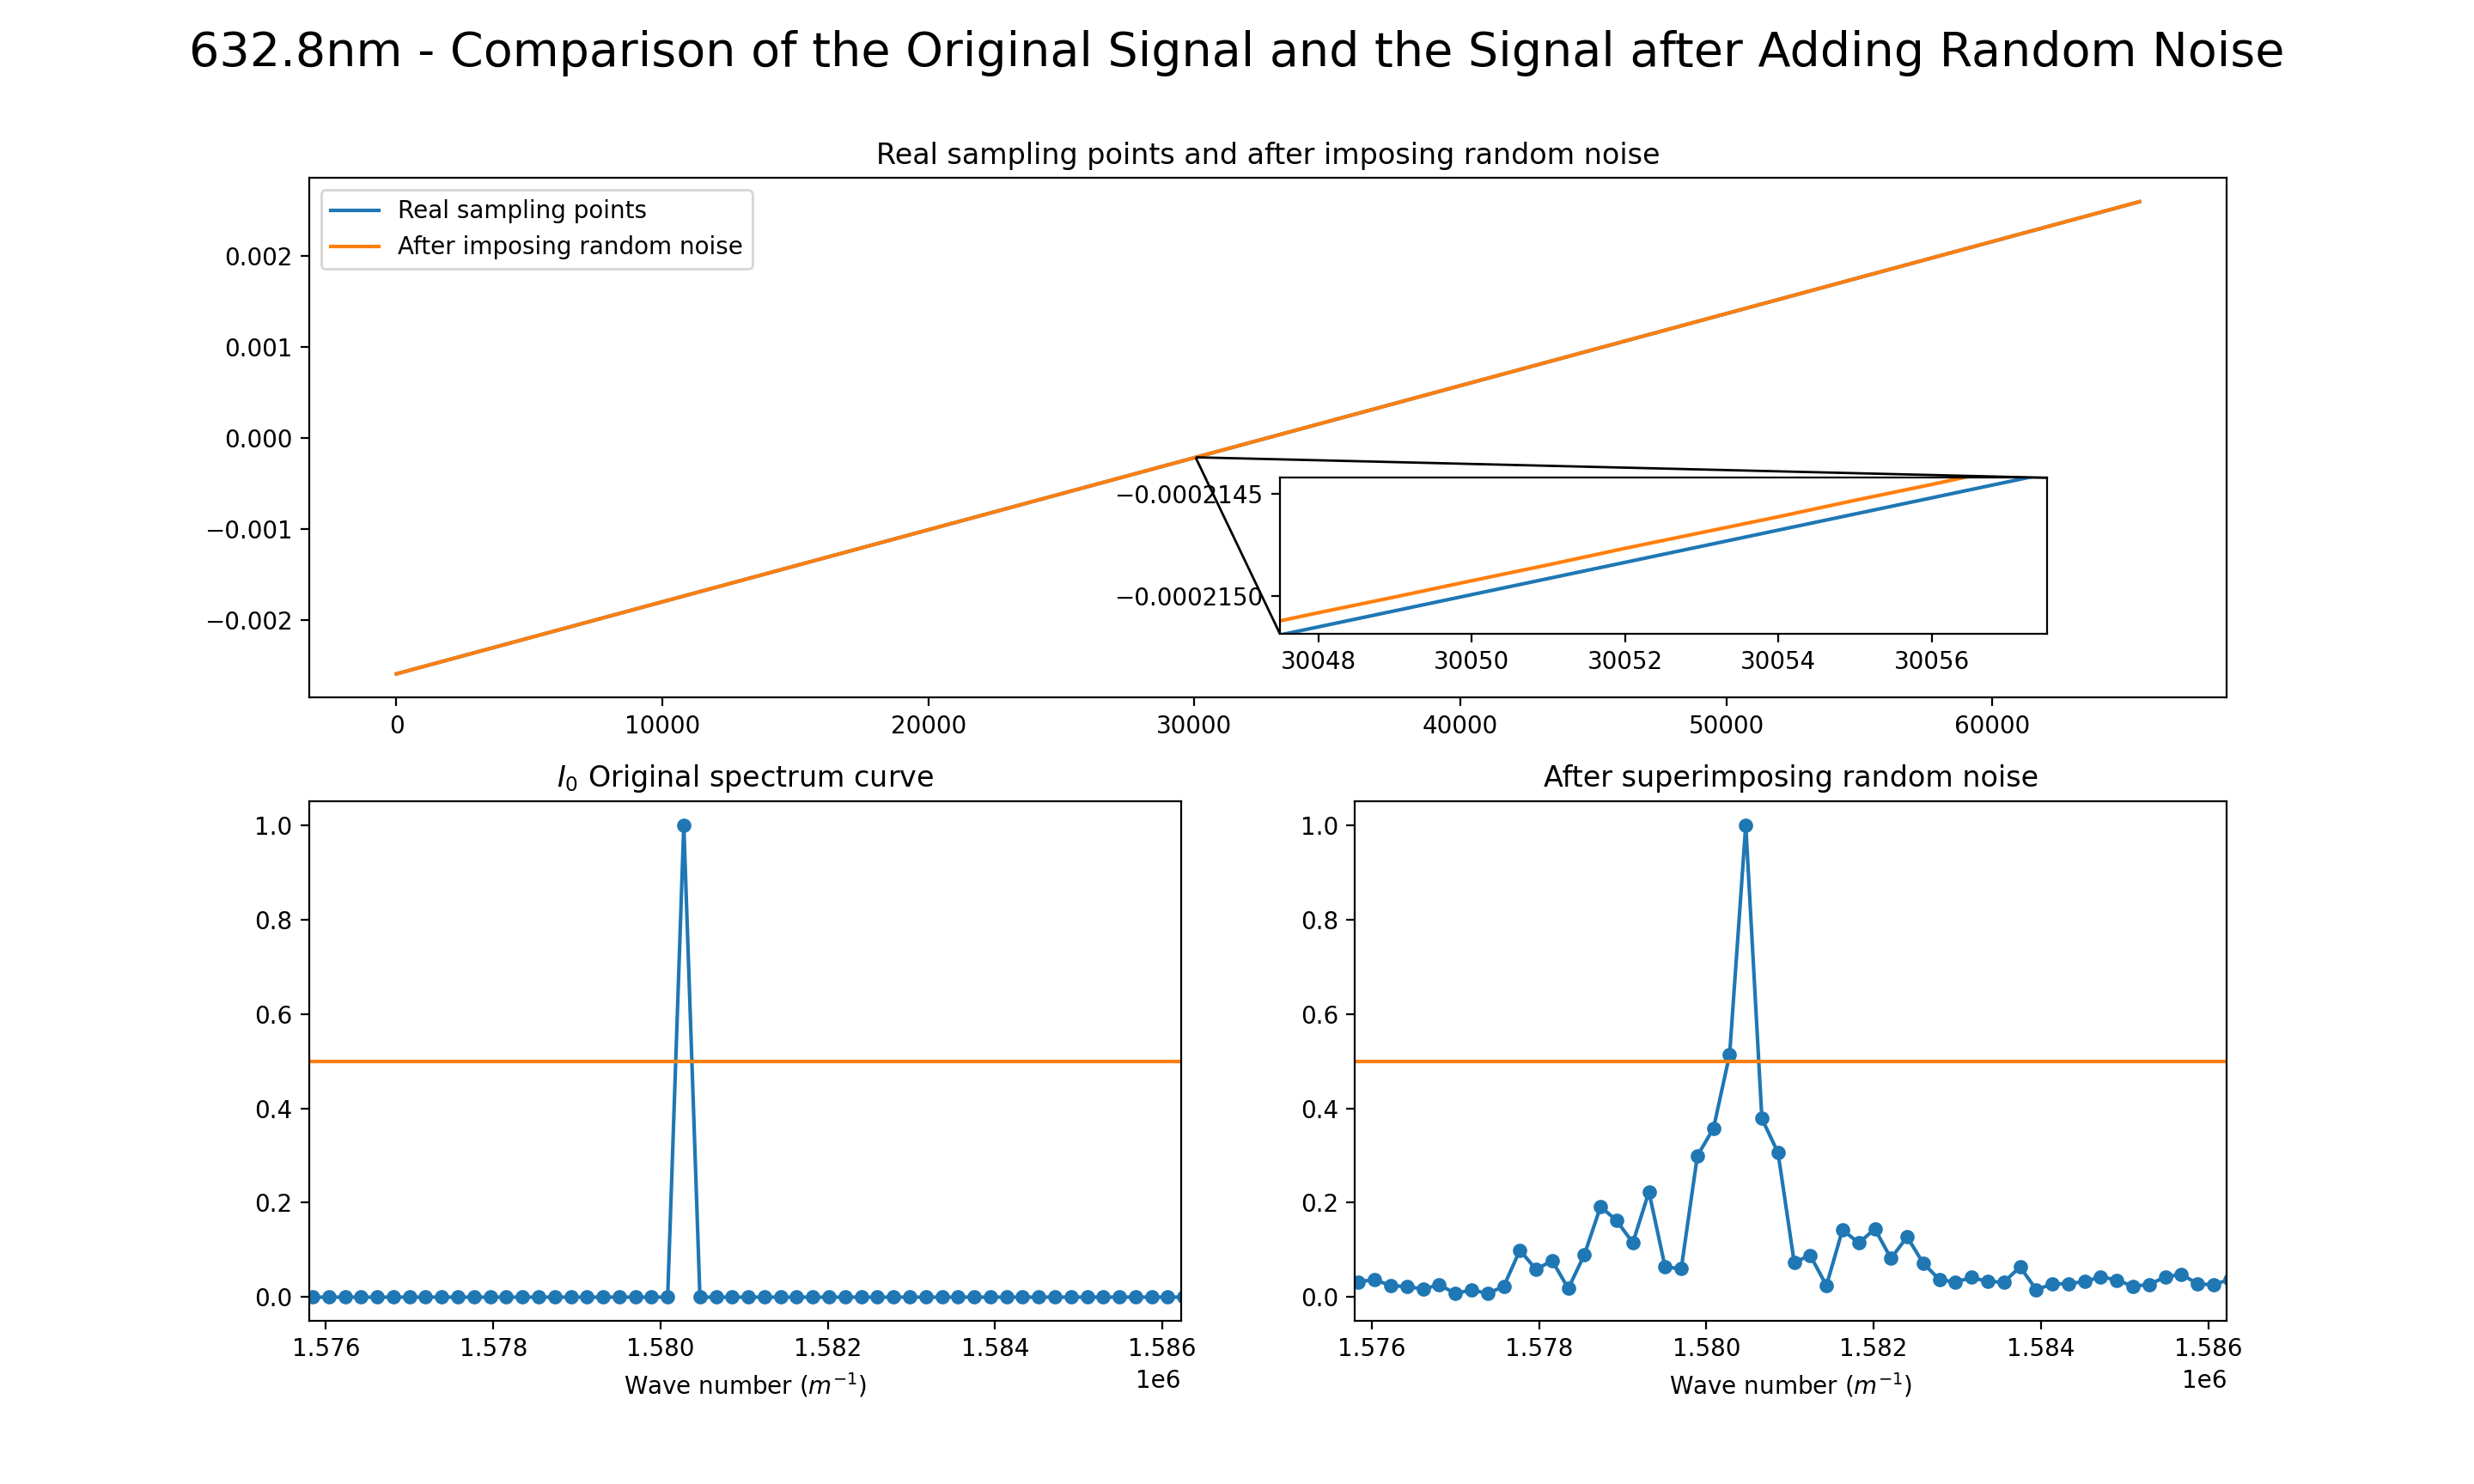
\includegraphics[width=0.5\textwidth]{随机噪声叠加1.png}}
    \caption{随机噪声叠加结果1(图片第一行代表理论扫描距离与叠加多次噪声后的扫描距离的比较,第二行左半部分代表代表未添加累积噪声的光谱曲线图,右半部分代表添加累积随机噪声后的光谱曲线图。)}
    \label{pic21}
\end{figure}

\begin{figure}[htbp]
    \centerline{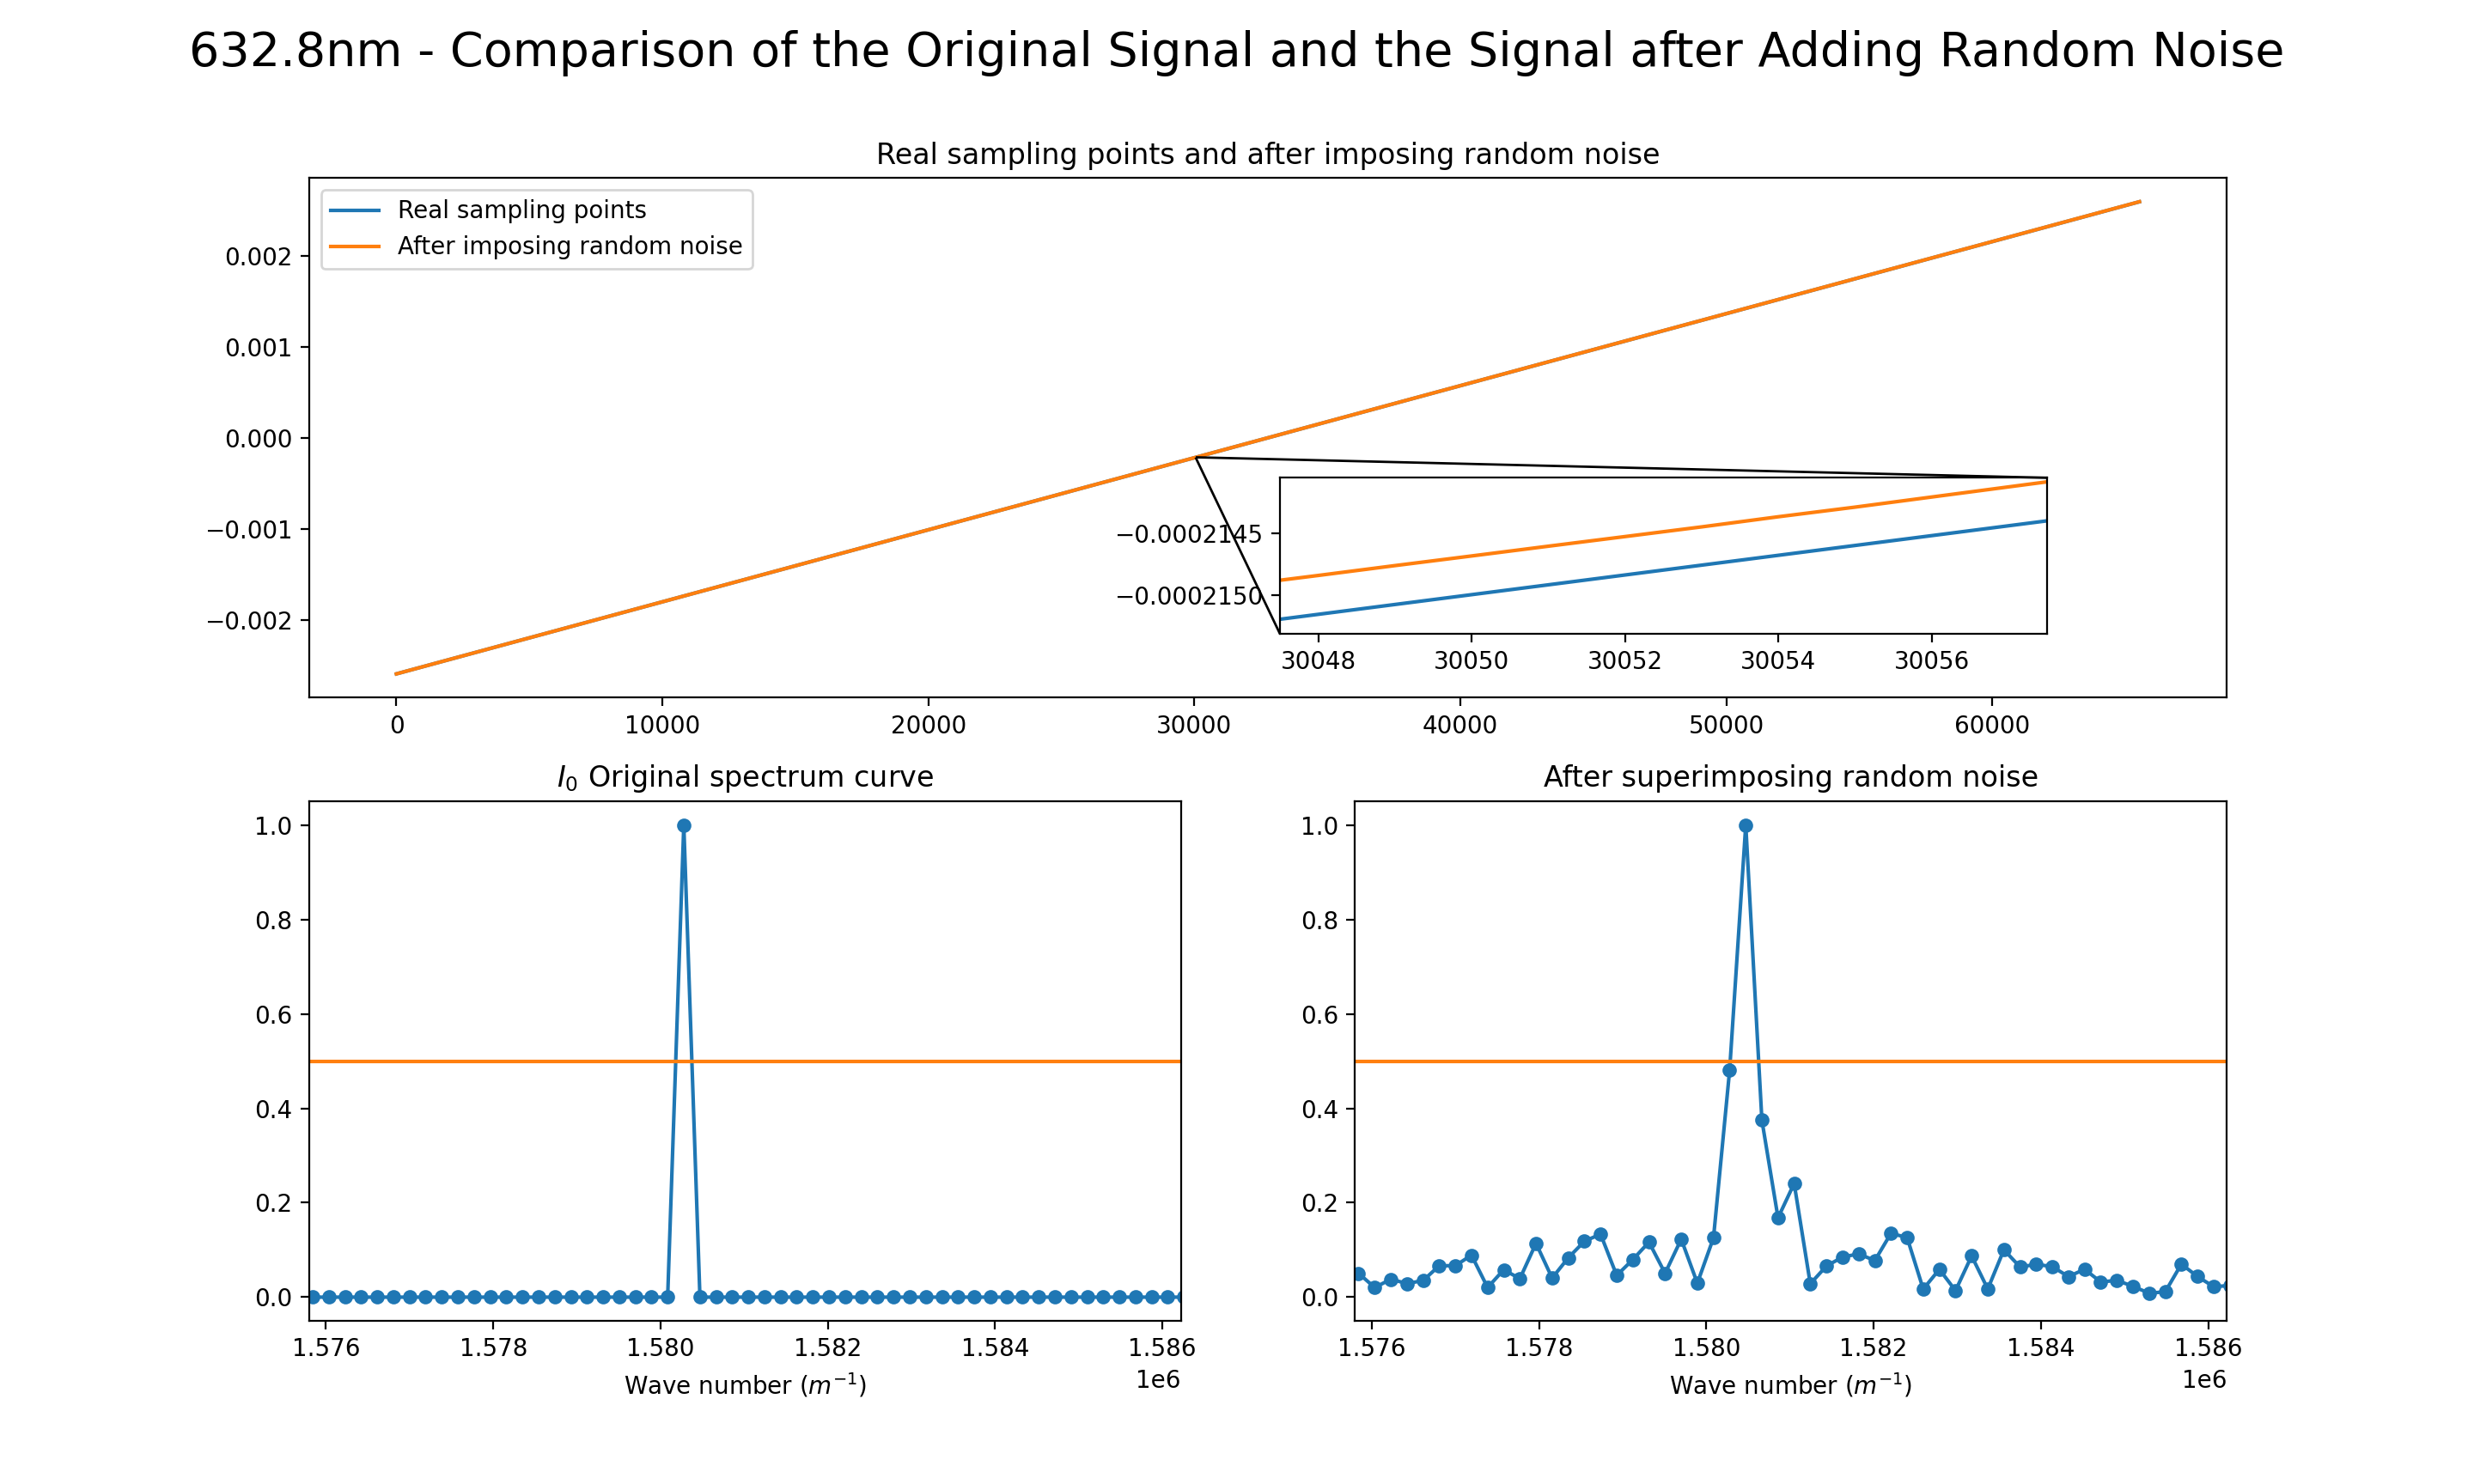
\includegraphics[width=0.5\textwidth]{随机噪声叠加2.png}}
    \caption{随机噪声叠加结果2(图片第一行代表理论扫描距离与叠加多次噪声后的扫描距离的比较,第二行左半部分代表代表未添加累积噪声的光谱曲线图,右半部分代表添加累积随机噪声后的光谱曲线图。)}
    \label{pic22}
\end{figure}

\begin{figure}[htbp]
    \centerline{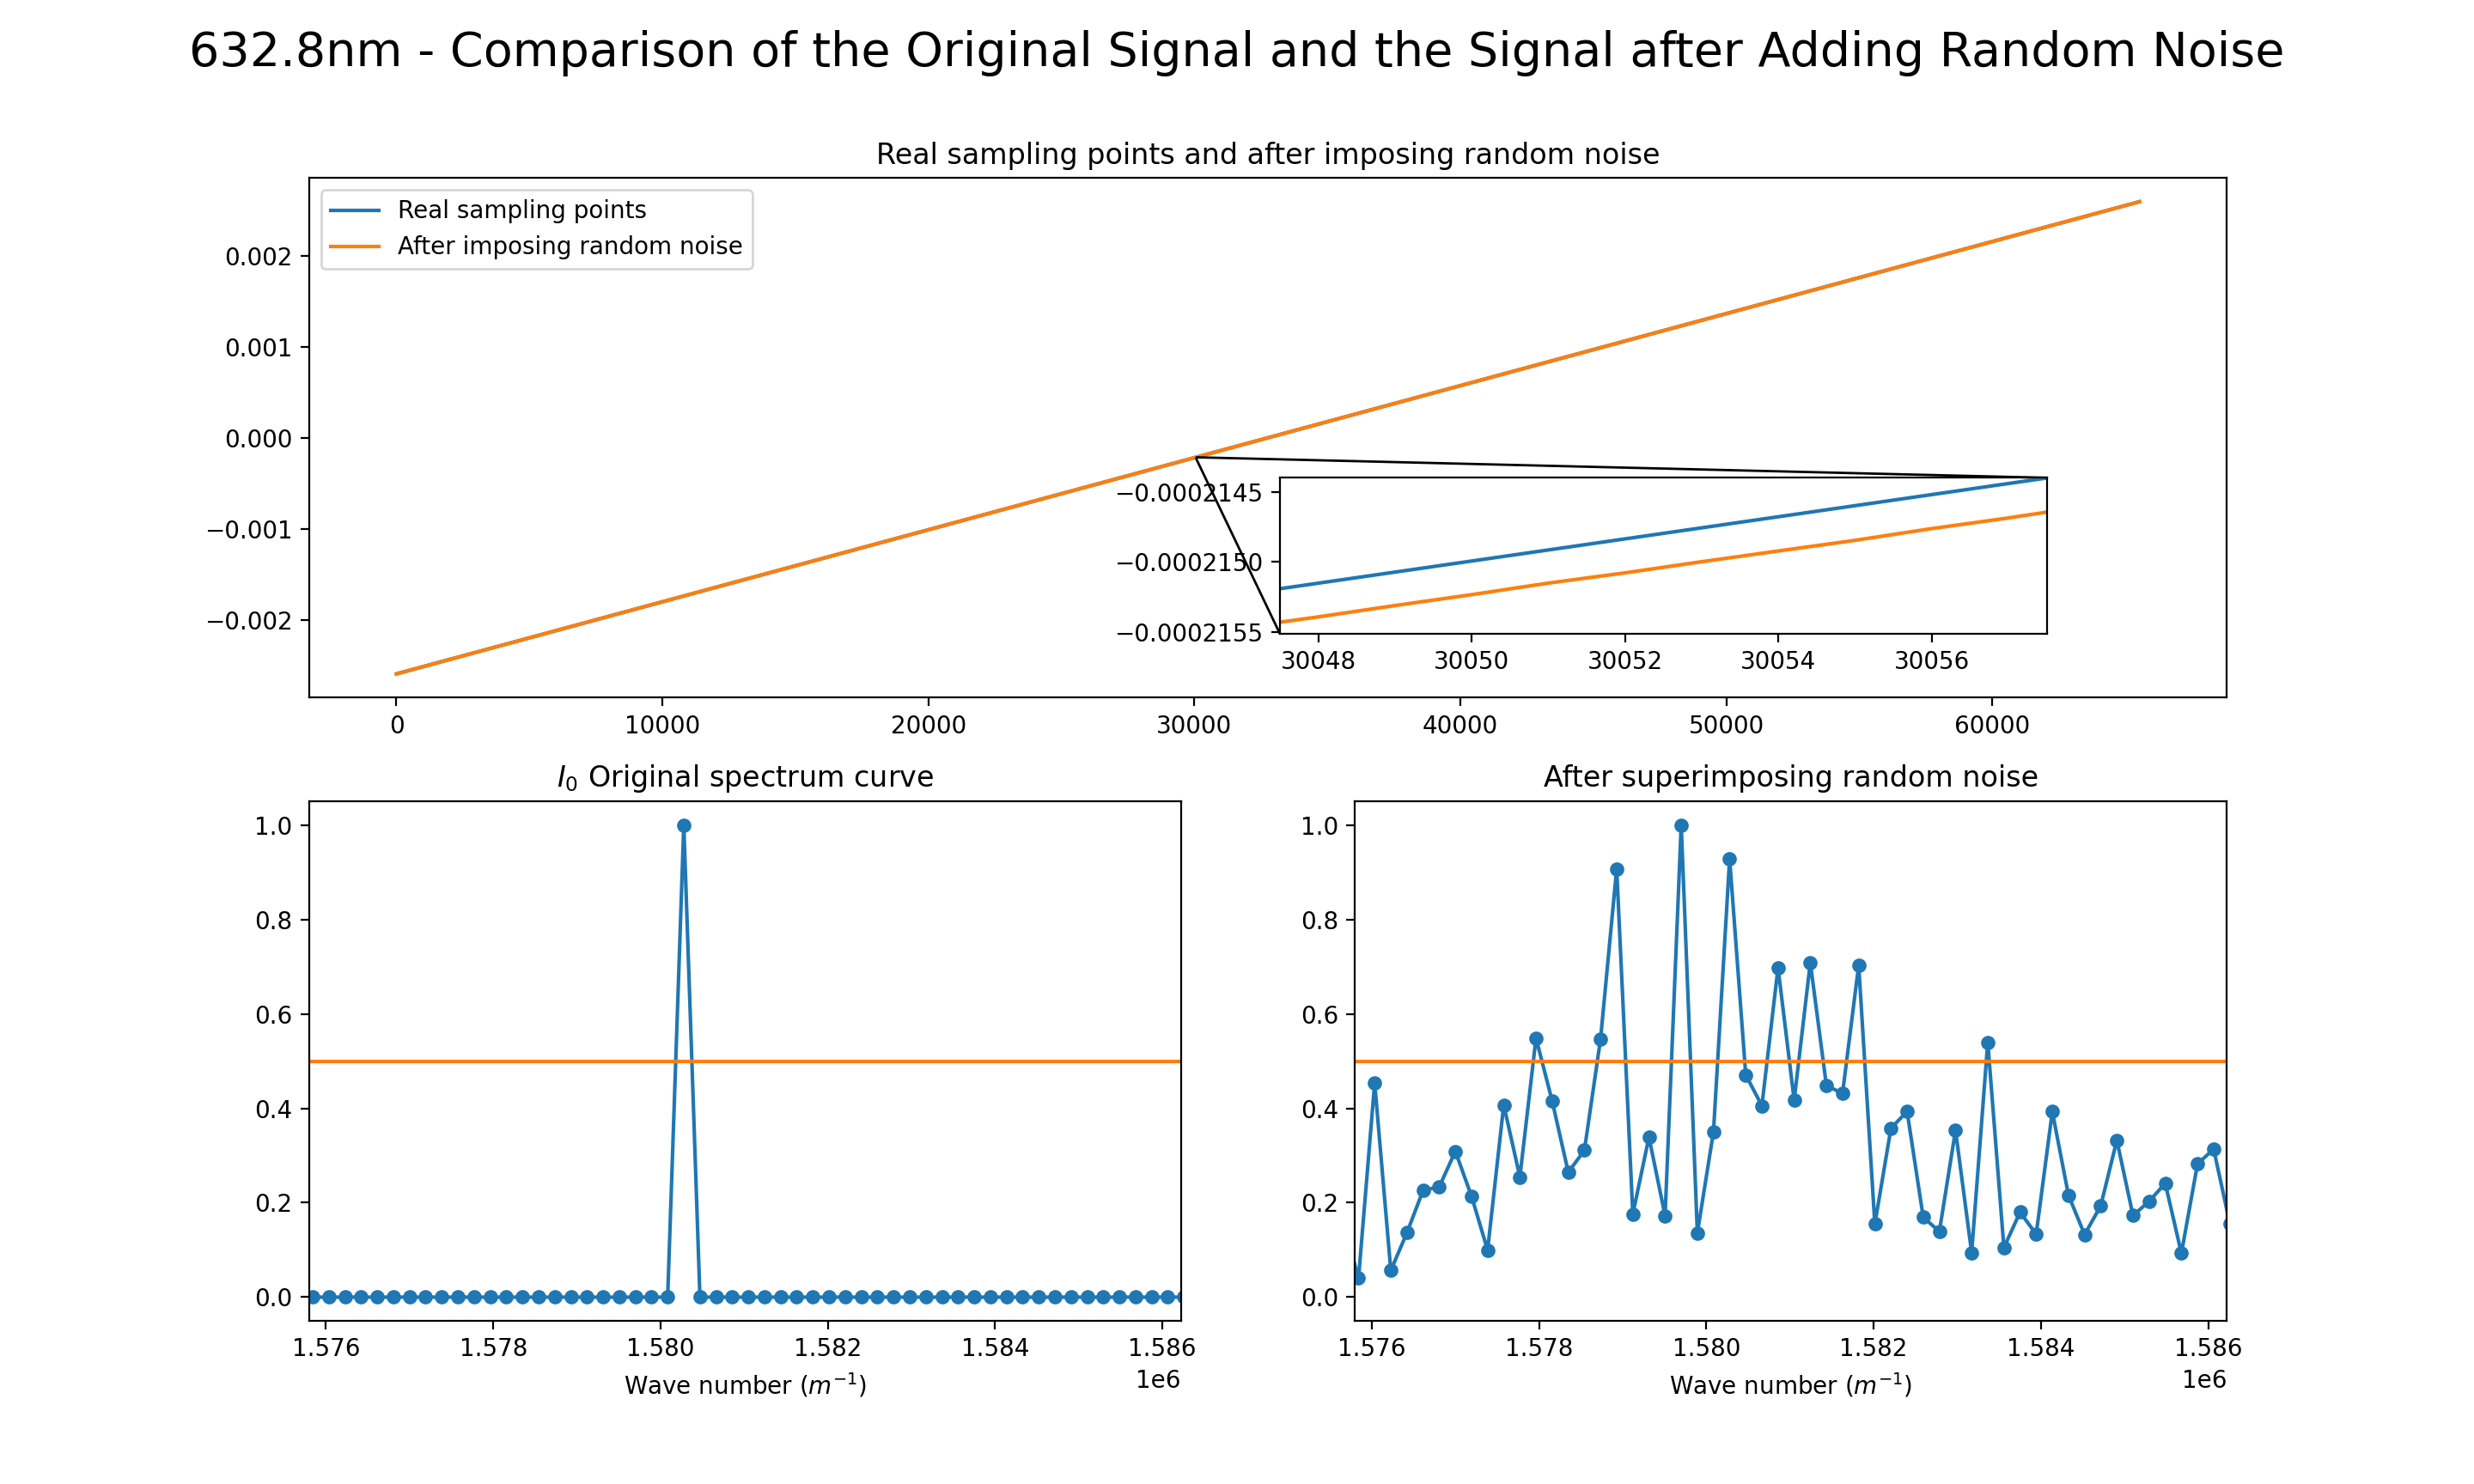
\includegraphics[width=0.5\textwidth]{随机噪声叠加3.png}}
    \caption{线性噪声叠加结果3(图片第一行代表理论扫描距离与叠加多次噪声后的扫描距离的比较,第二行左半部分代表代表未添加累积噪声的光谱曲线图,右半部分代表添加累积随机噪声后的光谱曲线图。)}
    \label{pic23}
\end{figure}

\begin{figure}[htbp]
    \centerline{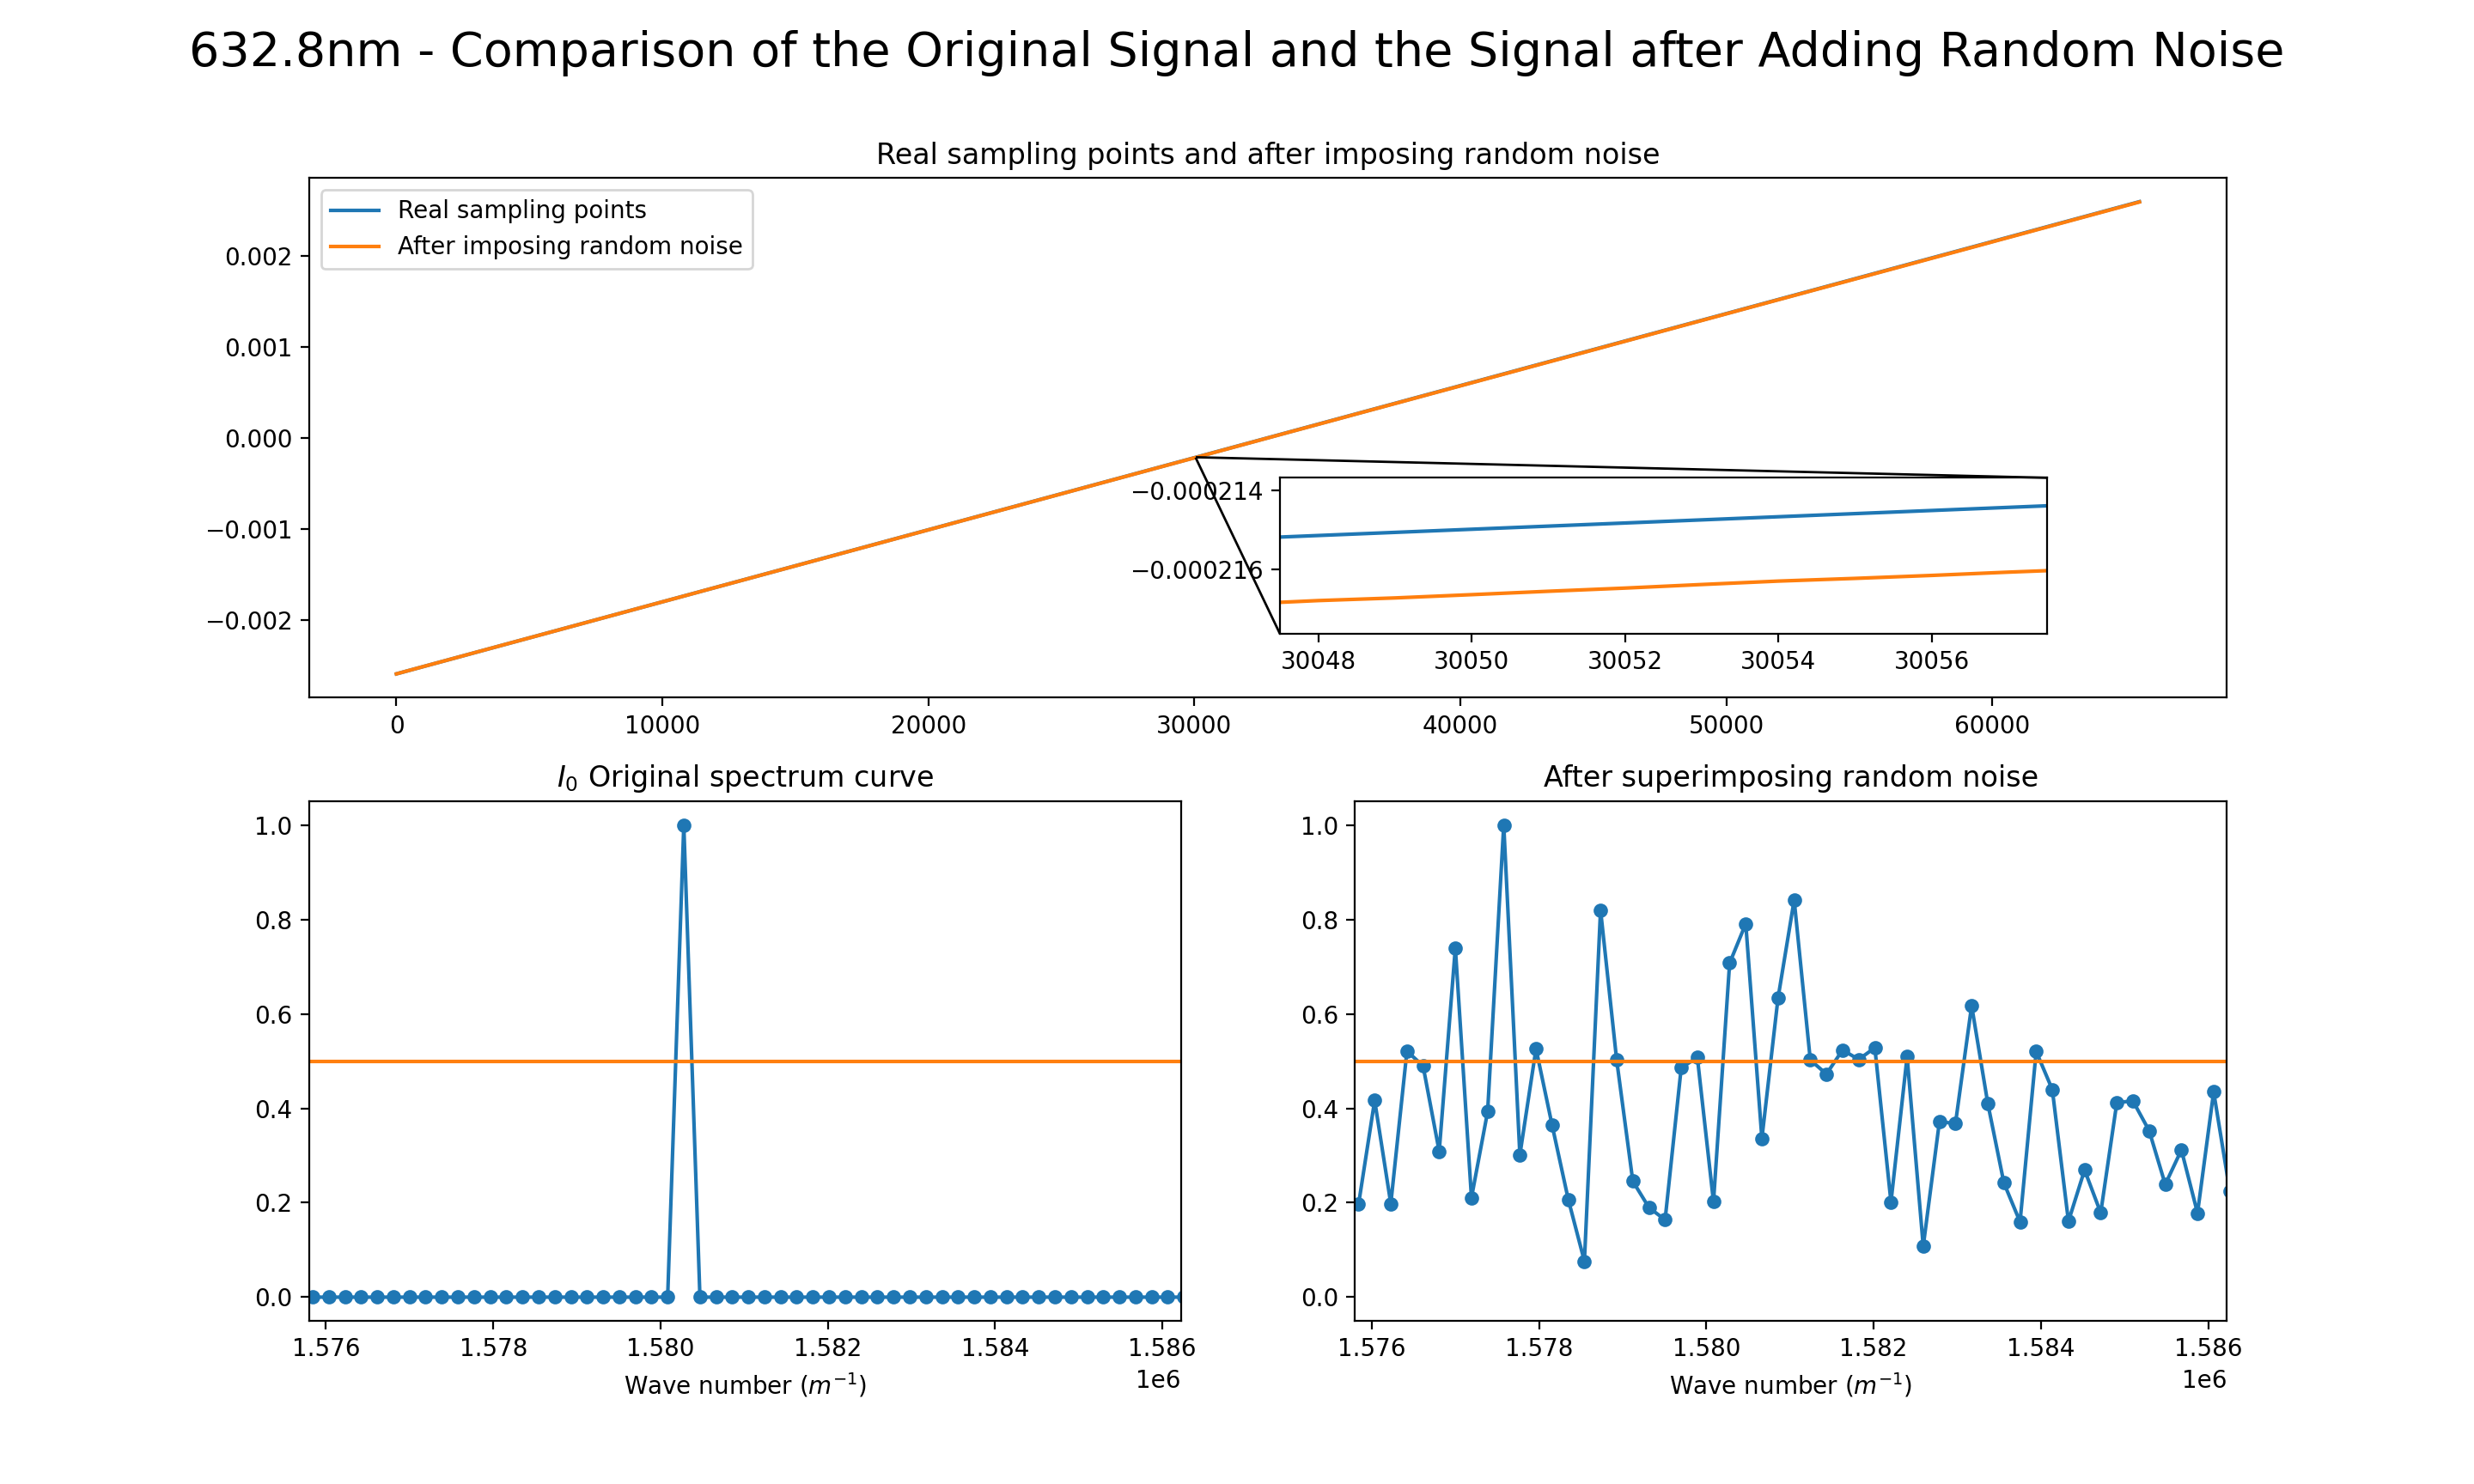
\includegraphics[width=0.5\textwidth]{随机噪声叠加4.png}}
    \caption{线性噪声叠加结果4(图片第一行代表理论扫描距离与叠加多次噪声后的扫描距离的比较,第二行左半部分代表代表未添加累积噪声的光谱曲线图,右半部分代表添加累积随机噪声后的光谱曲线图。)}
    \label{pic24}
\end{figure}

图片\ref{pic21}、图\ref{pic22}、图\ref{pic23}与图\ref{pic24}的结果表明,累积的随机误差会对光谱曲线的分辨率产生巨大的影响,一个极小的随机误差在不断迭代多次后会产生质的飞跃,具体表现在加噪声后的光谱曲线图的半峰全宽相比于原始光谱曲线图的半峰全宽加宽了较为大的范围。同时影响随着随机噪声幅度的增大而逐渐剧烈。

\section{结语}
本实验完成了利用Python仿真同时考虑有限扫描长度和采样间隔误差两因素影响下的傅里叶变换光谱测量系统的光谱测量曲线。仿真同时还分析了累积误差的叠加对傅立叶变换光谱测量曲线的影响。

\end{document}
